\chapter{Results}
\label{ch:results_discussion}

Testing the software is one part, testing its performance on real-world scenarios an other. The following sections give a few metrics of Graphinius as of the time of this writing.

\section{Size of the codebase}
\label{sect:complexity}

Lines of codes never accurately measure the complexity involved in a software project, as different languages and programming styles produce very diverging measures in that area (Java e.g. being much more ceremonial than Ruby or JavaScript). Nevertheless, here are the metrics in LOCs for the different parts of Graphinius as of May, 2nd, 2016, amounting to a total of 11,858 lines of code:

	\subsection{GraphiniusJS}
	\label{ssect:metrics_graphinius_js}
	
	The core JS library was split into source code as well as testing code, with the testing code again split into 3 different categories: 1) Synchronous tests are the ones that run fast enough so they can be continually re-executed on every file save, 2) Asynchronous test code for testing graph instantiation via remote file loading, and 3) Performance test code loading different graphs and executing some basic algorithms on them, measuring the time at every step.\\
	\textbf{Source code:} 2,557 LOC \\
	\textbf{Test code synchronous:} 5,160 LOC \\
	\textbf{Test code, asynchronous:} 321 LOC \\
	\textbf{Test code, performance:} 76 LOC \\	
	\textbf{Total:} 8,114 LOC.
	
	\subsection{Graph extraction demo code}
	\label{ssect:metrics_graphinius_graph_ext}
	
	The Anonymization demo library building on top of GraphiniusJS is split into source as well as synchronous test code, there was no need to introduce asynchronous test code in its case.\\	
	\textbf{Source code:} 602 LOC \\
	\textbf{Test code synchronous:} 448 LOC \\	
	\textbf{Total:} 1,050 LOC	
	
	\subsection{Social network anonymization demo code}
	\label{ssect:metrics_graphinius_anonym}
	
	The Anonymization demo library building on top of GraphiniusJS is split into source as well as synchronous test code, there was no need to introduce asynchronous test code in its case.\\	
	\textbf{Source code:} 778 LOC \\
	\textbf{Test code synchronous:} 455 LOC \\	
	\textbf{Total:} 1,233 LOC	
	
	\subsection{GraphiniusVIS}
	\label{ssect:metrics_graphinius_vis}
	
	The visualization library was written in pure JavaScript instead of TypeScript and due to its optical nature does not feature any automated test suite. \\	
	At the time of this writing the code base comprises 1,461 lines of code.
	

\section{Test coverage (just Graphinius JS)}
\label{sect:test_coverage}

Testing is a great practice to guide the development and programming effort while conducting a software project, but it is of equal importance as a documentation tool allowing the technical staff to demonstrate to their clients (customers and managers alike) the care they exercised in constructing their codebase. Coverage testing detects if parts of the codebase were either just partly tested or not tested at all, taking into account LOC coverage, percentage of functions / methods invoked as well as branch or general statement coverage.

As can be seen in Figure~\ref{fig:test_coverage}, Graphinius JS has been exhaustively tested, reaching 100\% coverage for all but the branches department. The lower value in this section is a result of \textit{else-branches} not taken, in cases when there was no \textit{else-branch} to take. This can be remedied by re-writing all \textit{if-statements} in the form of \textit{(boolean condition \&\& consequent)}, so that the code coverage tool does not recognize the \textit{if} keyword. The author has successfully tested this practice on the PFS.ts file (as can be seen in Figure~\ref{fig:test_coverage}) but at the time of this writing considers it inappropriate to alter perfectly good code throughout the library just for the sake of artificially achieving 100\% coverage.

\begin{figure}[ht]
	% \centering
	\hspace*{-0.5cm}
	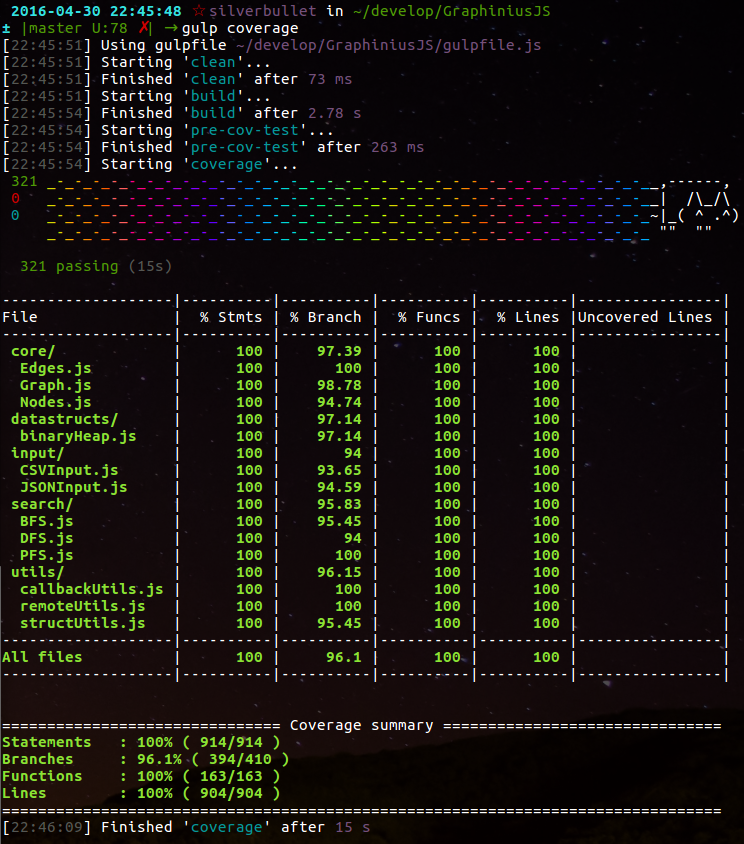
\includegraphics[width=1.1\textwidth]{figures/test_coverage}
	\caption{GraphiniusJS test coverage}
	\label{fig:test_coverage}
\end{figure}


%\section{Performance compared to selected libraries}
%\label{sect:perf_other_libs}

%	\subsection{iGraph (c++)}
%	\label{ssect:perf_igraph}
%	
%	\subsection{Graph Tool}
%	\label{ssect:perf_graphtool}
%	
%	\subsection{NetworkX (pure python)}
%	\label{ssect:perf_networkx}
%	
%	\subsection{Graphinius JS}
%	\label{ssect:perf_graphinius}
	

\section{Execution speed in various scenarios}
\label{sect:performance}

	All tests were executed on the author's Sandy Bride Quad Core i5, 8GB RAM, Ubuntu 16.04LTS, NodeJS version 5.5.0, bash console. All graphs were given as a simple CSV edge list. Experiments were run 10 times and average times (in milliseconds) taken; the measurements were conducted via JavaScript which translates to system real time (including all other processes running). The respective system time (only this process) was measured by the Unix \textit{time} utility and refers to a whole 'run', that means all of computations listed above it in sequence:
	
	\subsection{Sample graph 1}
	\label{ssect:sample_graph_1}
	
	The first sample graph consisted of 19,878 nodes and 49,062 edges:\\
	\textbf{Time to instantiate:} 450ms\\
	\textbf{Calculating degree distribution:} 28ms\\
	\textbf{Calculating BFS:} 265ms\\
	\textbf{Calculating degree distribution:} 260ms\\
	\textbf{Average system time:} 48ms
	
	\subsection{Sample graph 2}
	\label{ssect:sample_graph_2}
	
	The first sample graph consisted of 52,537 nodes and 140,868 edges:\\
	\textbf{Time to instantiate:} 1,260ms\\
	\textbf{Calculating degree distribution:} 51ms\\
	\textbf{Calculating BFS:} 680ms\\
	\textbf{Calculating degree distribution:} 790ms\\
	\textbf{Average system time:} 170ms
	
	\subsection{Sample graph 3}
	\label{ssect:sample_graph_3}
	
	The first sample graph consisted of 238,986 nodes and 797,115 edges:\\
	\textbf{Time to instantiate:} 7,703ms\\
	\textbf{Calculating degree distribution:} 208ms\\
	\textbf{Calculating BFS:} 3568ms\\
	\textbf{Calculating degree distribution:} 4993ms\\
	\textbf{Average system time:} 454ms\\


\section{Closing remarks about competitor libraries}
\label{sect:remarks_competitors}

The author contemplated writing a whole chapter about performance comparisons with other graph libraries as there are many of them out there (BGL, iGraph, GraphTool, NetworkX, Loom, some old Java based libraries, etc.). However, given the fact that \textbf{none} of those libraries were designed to run inside a browser including tight integration with a real-time 3D, Open/WebGL based visualization library, such comparisons would have been meaningless in any situation in which a user would require a non-effort, easily-configurable platform as ours.

